\documentclass[]{article}

\usepackage{float}
\usepackage{graphicx}

\usepackage{titling}
\newcommand{\subtitle}[1]{%
  \posttitle{%
    \par\end{center}
    \begin{center}\large#1\end{center}
    \vskip0.5em}%
}

\begin{document}

\title{Lab 1}
\subtitle{CS M152A}
\author{Aman Agarwal \& Lowell Bander}

\maketitle

\section{FPGA Design Workflow}

\textit{Please explain in your report how the steps in the FPGA design workflow correspond to the steps in the actual implementation using the Xilinx ISE and simulation tools.}\\

%TODO: complete this section

\subsection{Design}

The design stage of the FPGA development workflow is done outside of the the Xilinx ISE and its simulation tools, for it solely consists of the drawing of logical schematics so that the designer may understand the higher level functioning of the module to be constructed.

\subsection{Implementation}

The hierarchical file structure is determined based on which modules depend on others. At the very top-level we have a test bench file, \texttt{tb.v} which is directly above a unit under test file, \texttt{nexys3.v}. Below that we have a sequencer file and a uart file, \texttt{seq.v} and \texttt{uart\_top.v}. The sequencer is composed of the register file, \texttt{seq\_rf.v} and the ALU unit which has add and multiply modules. The Uart module represents the interface to the computer where we see the output. The Uart module is only needed for testing so it is not a part of the sequencer module.

\subsection{Simulation}

Lorem ipsum.

\subsection{Logic Synthesis}

Lorem ipsum.

\subsection{Technology Mapping}

Lorem ipsum.

\subsection{Cell Placement}

Lorem ipsum.

\subsection{Route}

Lorem ipsum.

\subsection{Bitstream Generation}

Lorem ipsum.

\section{Example Program}

\begin{table}[H]
\centering
\begin{tabular}{ l | l }
\textbf{Sequencer Instruction} & \textbf{Binary}\\\hline
\texttt{PUSH R0 0x4} & \texttt{0000 0010}\\
\texttt{PUSH R0 0x0} & \texttt{0000 0000}\\
\texttt{PUSH R1 0x3} & \texttt{0001 0011}\\
\texttt{MULT R0 R1 R2} & \texttt{1000 0110}\\
\texttt{ADD R2 R0 R3} & \texttt{0110 0011}\\
\texttt{PUSH R0 0x4} & \texttt{0000 0100}\\
\texttt{SEND R0} & \texttt{1100  xxxx}\\
\texttt{SEND R1} & \texttt{1101  xxxx}\\
\texttt{SEND R2} & \texttt{1110  xxxx}\\
\texttt{SEND R3} & \texttt{1111  xxxx}\\
\end{tabular}
\caption{Sequencer instructions translated to binary. The four least significant bits are ``don't care'' as their value is not used for the \texttt{SEND} instruction.}
\label{table:translation}
\end{table}

\begin{figure}[H]
\centering
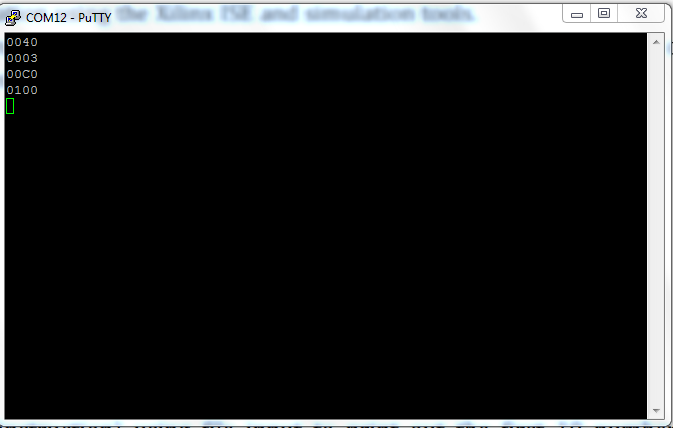
\includegraphics[width=10cm]{translation.PNG}
\caption{UART console output resulting from the executions in Table~\ref{table:translation}.}
\end{figure}

\section{Fibonacci}

For this section, we generated the first 10 Fibonacci numbers by writing the necessary sequencer instructions, translating them into machine instructions, and then loading them into the simulator using the \texttt{\$fopen} and \texttt{\$fscanf}.

\begin{table}[H]
\centering
\begin{tabular}{ l | l }
\textbf{Sequencer Instruction} & \textbf{Binary}\\\hline
\texttt{PUSH R0 0x0} & \texttt{0000 0000}\\
\texttt{PUSH R1 0x1} & \texttt{0001 0001}\\
\texttt{SEND R0} & \texttt{1100 xxxx}\\
\texttt{SEND R1} & \texttt{1101 xxxx}\\
\texttt{ADD R0 R1 R2} & \texttt{0100 0110}\\
\texttt{SEND R2} & \texttt{1110 xxxx}\\
\texttt{ADD R1 R2 R0} & \texttt{1001 1000}\\
\texttt{SEND R0} & \texttt{1100 xxxx}\\
\texttt{ADD R2 R0 R1} & \texttt{1010 0001}\\
\texttt{SEND R1} & \texttt{1101 xxxx}\\
\texttt{ADD R0 R1 R2} & \texttt{0100 0110}\\
\texttt{SEND R2} & \texttt{1110 xxxx}\\
\texttt{ADD R1 R2 R0} & \texttt{1001 1000}\\
\texttt{SEND R0} & \texttt{1100 xxxx}\\
\texttt{ADD R2 R0 R1} & \texttt{1010 0001}\\
\texttt{SEND R1} & \texttt{1101 xxxx}\\
\texttt{ADD R0 R1 R2} & \texttt{0100 0110}\\
\texttt{SEND R2} & \texttt{1110 xxxx}\\
\texttt{ADD R1 R2 R0} & \texttt{1001 1000}\\
\texttt{SEND R0} & \texttt{1100 xxxx}\\
\texttt{ADD R2 R0 R1} & \texttt{1010 0001}\\
\end{tabular}
\caption{The sequencer instructions, and their corresponding machine translations, necessary to generate the first 10 Fibonacci numbers. When loaded into simulation, the ``don't care'' values were substituted for \texttt{0}, but it is important to note that we could have just as easily used \texttt{1}.}
\label{table:fib}
\end{table}

\begin{figure}[H]
\centering
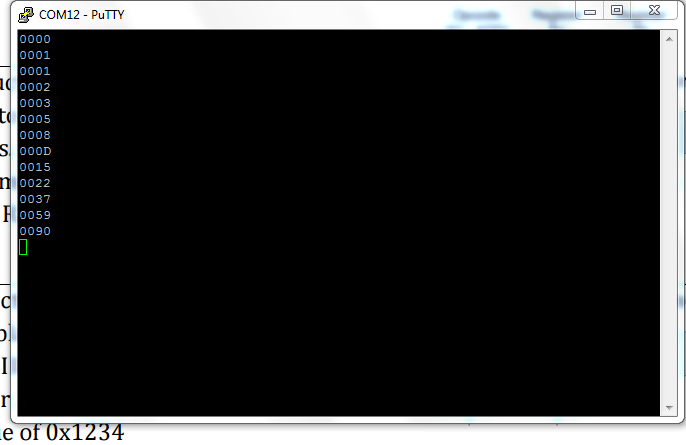
\includegraphics[width=10cm]{fib.PNG}
\caption{UART console output resulting from the executions in Table~\ref{table:fib}.}
\end{figure}

\section{Exercise 1}

%TODO: complete this section

\subsection{Clock Enable}
\begin{enumerate}
\item 
\item 
\item 
\item 
\end{enumerate}
\subsection{Instruction Valid}
\begin{enumerate}
\item 
\item 
\item 
\item 
\item 
\end{enumerate}
\subsection{Register File}
\begin{enumerate}
\item 
\item 
\item 
\item 
\item 
\end{enumerate}

\section{Exercise 2}

%TODO: complete this section

\subsection{Nicer UART Output}
\subsection{An Easier Way to Load Sequencer Program}

\begin{enumerate}
\item 
\item
\end{enumerate}

\begin{enumerate}
\item 
\item
\item
\end{enumerate}

\subsection{Fibonacci Numbers}

\end{document}